\documentclass[12pt, a4paper, oneside]{book}
\usepackage[utf8]{inputenc}
\usepackage[spanish]{babel}
\usepackage{amsmath}
\usepackage{amsfonts}
\usepackage{amssymb}
%\usepackage{makeidx}
\usepackage{graphicx}
\usepackage{csquotes}
\usepackage{tikz}
%\usepackage{lmodern}
%\usepackage{kpfonts}
\usepackage[left=2cm,right=2cm,top=2cm,bottom=2cm]{geometry}
\usepackage{bm}
%\usepackage{cite}
\usepackage[
backend = biber,
bibstyle = apa,
citestyle = numeric, 
sorting = none
]{biblatex}
\usepackage{hyperref}
\usepackage{cleveref}
%\usepackage{autonum}
%\usepackage{comment}
\usepackage{braket}
\usepackage{amsthm}
\usepackage{csquotes}
\usepackage{physics}
\usepackage{fancyhdr}
\usepackage{newtxtext}
\usepackage{newtxmath}
\usepackage{subcaption}
\usepackage[bottom]{footmisc}
\usepackage{fancyhdr}

\graphicspath{{FIGURAS/}}
\addbibresource{falso_vacio.bib}

\usetikzlibrary{babel}

%\numberwithin{equation}{section}

\DeclareFieldFormat{labelnumberwidth}{\mkbibbrackets{#1}}

\defbibenvironment{bibliography}
  {\list
     {\printtext[labelnumberwidth]{%
      \printfield{labelprefix}%
      \printfield{labelnumber}}}
     {\setlength{\labelwidth}{\labelnumberwidth}%
      \setlength{\leftmargin}{\labelwidth}%
      \setlength{\labelsep}{\biblabelsep}%
      \addtolength{\leftmargin}{\labelsep}%
      \setlength{\itemsep}{\bibitemsep}%
      \setlength{\parsep}{\bibparsep}}%
      \renewcommand*{\makelabel}[1]{\hss##1}}
  {\endlist}
  {\item}

\linespread{1.6}

\allowdisplaybreaks

\decimalpoint

%\clearpage\null\thispagestyle{empty}

\begin{document}
	
\frontmatter
	
\begin{titlepage}
\begin{center}

\thispagestyle{empty}

\textsc{\LARGE{Universidad Nacional Mayor de San Marcos}} \\
\large{Universidad del Perú, Decana de América} \\ [0.5cm] 
\textsc{\LARGE Facultad de Ciencias Físicas} \\  
\textsc{\Large Escuela Profesional de Física} \\ [1cm]

\includegraphics*[height = 5cm]{unmsm_logo.png} \\ [1cm]

\textsc{\LARGE Trabajo de Investigación} \\ [0.25cm]
\large \text{Para optar por el grado académico de Bachiller en Física} \\ [0.5cm]

\LARGE{\bfseries{Decaimiento del falso vacío en la Mecánica Cuántica y la Teoría Cuántica de Campos}} \\ [0.5cm] 

\textsc{\LARGE Autor} \\ [0.25cm] 
\large{Erwin Renzo Franco Diaz} \\ [0.5cm]

\textsc{\LARGE Asesor} \\ [0.25cm] 
\large{Teófilo Vargas Auccalla} \\ 

\vfill

\large \text{Lima, Perú} \\ [0.25cm]
\large \text{Julio 2021}

\end{center}
\end{titlepage}

\newgeometry{top = 1in, bottom = 1in, right = 1in, left = 1in}

\addcontentsline{toc}{chapter}{Resumen}

\begin{center}
	\thispagestyle{plain}
	\setlength{\parskip}{0pt}
	{\huge{\textsc{Resumen}} \par}

\end{center}

\noindent
Clásicamente, es bien sabido que una partícula que se encuentra en un potencial que cuenta con dos mínimos distintos, es estable en cualquiera de estos. Esto deja de ser cierto al considerar una partícula cuántica puesto que existe una cierta probabilidad de que, si se encuentra inicialmente en el mínimo de mayor energía, decaiga al de menor. Es decir, el potencial cuenta con un falso vacío.  En el presente trabajo de investigación se realizará un análisis detallado y sistemático del decaimiento del falso vacío en ausencia de la gravedad. Inicialmente, se estudia este fenómeno 
en la Mecánica Cuántica, estableciendo su relación con el efecto túnel y la aproximación WKB. Haciendo uso de la 
%aproximación semiclásica WKB 
integral de camino euclideana y la aproximación del punto estacionario, se obtiene una expresión analítica para la tasa de decaimiento del falso vacío $\Gamma$ a primer orden en $\hbar$.
%del tiempo euclidiano. 
Posteriormente, se generaliza este formalismo para la Teoría Cuántica de Campos del campo escalar. Se demostrará que, en este caso, el decaimiento del falso vacío tiene como resultado la nucleación y evolución de una burbuja de verdadero vacío en el espaciotiempo de Minkowski.

\hfill

\noindent
\textbf{Palabras claves:} falso vacío, tasa de decaimiento, bounce, burbuja.

%\colorbox{yellow}{añadir descripcion de capitulos}	

\newpage

\addcontentsline{toc}{chapter}{Abstract}

\begin{center}
	\thispagestyle{plain}
	\setlength{\parskip}{0pt}
	{\huge{\textsc{Abstract}} \par}
	
\end{center}

\noindent
Classically, it is well known that a particle in a potential with two different minima, is stable in any of these. This is no longer true for a quantum particle since there is a certain probability that, if it is initially in the minimum with higher energy, decays into the lower. This means that the potential has a false vacuum. The main objetive of this work is to develop a detailed and systematic analysis of false vacuum decay in the absence of gravity. At first, this phenomenon is studied in Quantum Mechanics in order to stablish its relation with the tunneling effect   and the WKB approximation. Using the euclidean path integral and the stationary point approximation, an analytic expression for the false vacuum decay rate $\Gamma$ is obtained to first orden in $\hbar$.
%del tiempo euclidiano. 
Then, this formalism is extended to the Quantum Field Theory of the scalar field. It will be demonstrated that, in this case, false vacuum decay results in the nucleation and evolution of a true vacuum bubble in Minkowski spacetime.

\hfill

\noindent
\textbf{Keywords:} false vacuum, decay rate, bounce, bubble.

\newpage

\addcontentsline{toc}{chapter}{Agradecimientos}

\begin{center}
	\thispagestyle{plain}
	
	\setlength{\parskip}{0pt}
	{\huge{\textsc{Agradecimientos}} \par}
\end{center}

Primero, agradecer a mis padres por haber confiado en mí y haberme dado la oportunidad de poder estudiar esta maravillosa carrera, puesto que, sin su apoyo incondicional a lo largo de todos estos años, esto no hubiera sido posible. 

Agradecer a mi asesor, el profesor Teófilo Vargas Aucalla, por sus enseñanzas tanto en lo académico como en lo personal, así como por su incansable esfuerzo por el desarrollo de la Física Teórica en el Perú.  
%A pesar de lo difícil que puede resultar la Física, y en particular la Física Teórica, la libertad 
A su vez, también me gustaría agradecer a los profesores Fulgencio Villegas Silva y Jesús Sánchez Flores por las experiencias y enseñanzas compartidas. 

Agradecer a todos los compañeros que tuve el agrado de conocer, gracias a quienes las largas y arduas horas de estudio se hicieron más llevaderas. Si bien no pudimos compartir un salón de clases durante el último año, espero podamos reencontrarnos en un futuro no muy lejano. 

Por último, pero no por eso menos importante, agradecer a todas las autoridades, profesores y personal administrativo de la Universidad Nacional Mayor de San Marcos, y en especial de la Facultad de Ciencias Físicas que, a pesar de las grandes dificultades con las que se tienen que enfrentar día a día, hacen todo lo posible para brindar una formación de calidad a todos sus alumnos.
%llevar el correcto funcionamiento de la misma. 

\newpage

\addcontentsline{toc}{chapter}{Índice general}
\tableofcontents

\addcontentsline{toc}{chapter}{Índice de figuras}
\listoffigures

\newpage

\begin{center}
	\thispagestyle{empty}
	\hspace{0pt}
	\vfill
	\textit{Dedicado a .}
	\vfill
	\hspace{0pt}
\end{center}

\mainmatter

% Chapter Template

\chapter{Introducción} % Main chapter title

\section{Motivación}

Desde su formulación inicial en la década de 1920, se hizo evidente que la Mecánica Cuántica es una teoría radicalmente distinta al resto de la Física conocida hasta ese entonces. Uno de los ejemplos más sorprendentes de esto es el efecto túnel o tunelamiento. Descubierto inicialmente por George Gamow en 1928 para explicar el decaimiento alfa \cite{gamow1928quantum}, este fenómeno permite a una partícula atravesar una barrera de potencial, a pesar de que no pueda hacerlo clásicamente por no contar con la energía suficiente. 

Una consecuencia importante del efecto túnel es el decaimiento del falso vacío, tema principal a tratar en este trabajo. En este caso, la partícula atraviesa la barrera de potencial a la vez que decae al estado de mínima energía. 

El decaimiento del falso vacío tiene implicaciones importantes tanto en la física de partículas como en la cosmología. 

%$\Gamma$ que establece una escala temporal en la cual podría ocurrir. 

\section{Planteamiento del problema}

\colorbox{yellow}{revisar}
Consideremos un potencial como el de la figura \ref{fig:potencial} que posee dos mínimos distintos, uno mayor que otro. Clásicamente, ambos puntos son estables. Sin embargo, esta no es la situación a nivel cuántico. Debido al efecto túnel, existe la posibilidad de que una partícula que se encuentre inicialmente en $x_+$, atraviese la barrera %reapareciendo por $x_0$                                                            
al estado de menor energía del sistema. Es por esto que a $x_+$ se le denomina como falso vacío y a este proceso como decaimiento del falso vacío.

A lo largo del trabajo tomaremos la figura \ref{fig:potencial} como nuestro potencial de referencia. % al momento de realizar los cálculos. 

\begin{figure}[h!]
	\centering
	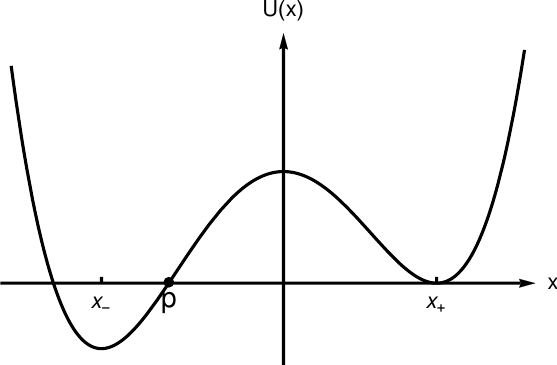
\includegraphics[scale = 0.4]{../FIGURAS/potencial}
	\caption{Potencial con un falso vacío en $x_+$ \cite{Ai:2019dqr}.}
	\label{fig:potencial}
\end{figure}

\section{Objetivo}

El objetivo principal del presente trabajo de investigación es el cálculo de la tasa de decaimiento del falso vacío $\Gamma$ a primer orden en $\hbar$. 
%para el estado metaestable de menor energía
Inicialmente se llevará a cabo en la Mecánica Cuántica haciendo uso de la integral de camino euclideana y la aproximación del punto estacionario siguiendo el formalismo planteado originalmente por Coleman y Callan \cite{coleman1977fate, callan1977fate}. %Primero se estudiará este fenómeno en la Mecánica Cuántica y luego en la Teoría Cuántica de Campos del campo escalar. 
Posteriormente el mismo será extendido a la Teoría Cuántica de Campos del campo escalar donde además se analizará la formación de burbujas de verdadero vacío y su evolución espaciotemporal. 




%\begin{figure}[h]
%	\centering
%	\begin{tikzpicture}[scale = 2]
%	
%	\draw[<->] (-2, 0) -- (2, 0) node[anchor = west] {$x$}; 
%	\draw[<->] (0,-1) -- (0,2) node[anchor = south] {$V(x)$};
%	
%	\draw[line width = 0.5mm, color = blue, domain = -1.5:1.5, smooth] plot(\x, {((\x - 1)^2)*((\x + 1)^2) - 0.2*(\x + 1)});
%	
%	\node[anchor = north] at (-1, 0) (a) {$a$};
%	\draw (-1,-0.05) -- (-1,0.05);
%	
%	\node[anchor = north] at (-1, 0) (a) {$a$};
%	\draw (-1,-0.05) -- (-1,0.05);
%	
%	\node[anchor = southleine] at (1, 0) (b) {$b$};
%	\draw (1,-0.05) -- (1,0.05);
%	\end{tikzpicture}
%	%\caption{Potencial para el estudio numérico del decaimiento del falso vacío. Cuenta con una región de falso (FV) y verdadero vacío (R), separados por una barrera (B) \cite{Masoumi:2015psa}.}
%	%\label{fig:potencial_numerico} 
%\end{figure}








\input{CAPITULOS/falso_vacio_qm}
\chapter[Decaimiento del falso vacío en la TCC]{Decaimiento del falso vacío en la Teoría Cuántica de Campos}

%\section{Soluciones a la ecuación de movimiento}

\section{Tasa de decaimiento del falso vacío por unidad de volumen
	%en la Teoría Cuántica de Campos
}

Consideremos el campo escalar $\phi\qty(x)$ cuya acción $S\qty[\phi\qty(x)]$ está dada por %\footnote{$x=\qty(t, x, y, z)$ es el cuadrivector posición.} 
\begin{equation} \label{eq:accion_qft}
S\qty[\phi\qty(x)] = \int \dd[4]{x} \qty[\frac{1}{2}\qty(\pdv{\phi}{t})^2 - \frac{1}{2}\qty(\grad{\phi})^2 - U\qty(\phi) ]
\end{equation}
donde el potencial 
%\footnote{$U\qty(\phi)$ es la densidad de potencial pero por comodidad no usaremos esta denominación.} 
$U\qty(\phi)$ está dado en la figura \ref{fig:potencial_qft}. Cuenta con dos mínimos $\phi_-$ y $\phi_+$, de los cuales este último es un falso vacío por lo que, al igual que en la Mecánica Cuántica, 
%revisar terminos: "se encuentre" o "tenga una configuracion"
esperamos que, si la configuración inicial del campo es $\phi_+$, 
exista una cierta probabilidad de que
pueda decaer a $\phi_-$ por tunelamiento. Resulta conveniente añadirle una constante 
%a $U\qty(\phi)$ 
de tal manera que $U\qty(\phi_+) = 0$ y la energía del campo en el falso vacío sea finita \cite{andreassen2017precision}. 
\begin{figure}[t]
	\centering
	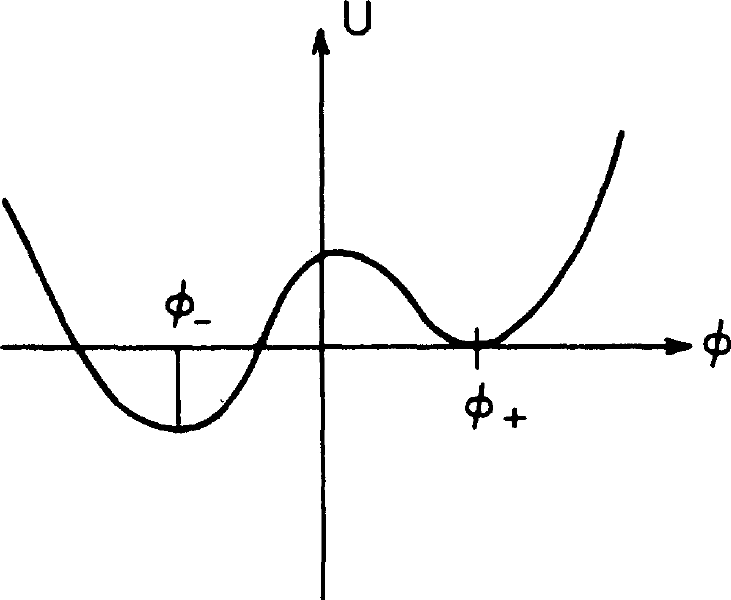
\includegraphics[scale=0.25]{FIGURAS/potencial_qft}
	\caption{Potencial en el que se encuentra el campo escalar dado por la acción \eqref{eq:accion_qft}. Notamos que cuenta con un falso vacío en $\phi_+$ \cite{callan1977fate}.}
	\label{fig:potencial_qft}
\end{figure}

A pesar de esto, la energía del campo en el verdadero vacío es infinita debido a que $U\qty(\phi_-)$ es distinto de cero e integramos sobre todo el espacio \cite{paranjape2017theory}. De la misma manera, la barrera de potencial a través de la cual se debe dar el tunelamiento, también es infinita, por lo que el decaimiento del falso vacío solo puede darse en ciertas regiones del espacio. 
%Como esta es arbitraria, la tasa de decaimiento es proporcional al volumen y por lo tanto, infinita \cite{weinberg2012classical}.  
%añadir algo sobre que la diferencia de energia respecto al falso vacio es finita
Es por esto que la cantidad físicamente relevante a calcular es la tasa de decaimiento del falso vacío por unidad de volumen $\Gamma/V$ \cite{weinberg2012classical} de la forma
\begin{equation} \label{eq:gamma_volumen_WKB}
\frac{\Gamma}{V} = Ae^{-B/\hbar}\qty(1 + \order{\hbar}),
\end{equation}
% serán discutidas más adelante. 
donde $A$ y $B$ son coeficientes a determinar mediante la extensión del formalismo desarrollado en el capítulo anterior a la Teoría Cuántica de Campos del campo escalar. 



\section{Bounces en la Teoría Cuántica de Campos}

%Habiendo desarrollado el formalismo 
Si bien al momento de calcular $\Gamma/V$ haremos uso del formalismo desarrollado en el capítulo anterior,
%adaptado, mediante analogía con lo estudiado 
previamente debemos plantear el problema clásico correspondiente con sus respectivas condiciones de frontera y encontrar 
%las configuraciones clásicas  
las configuraciones clásicas del campo que no son más que las soluciones a la ecuación de movimiento.  

Al aplicar el cambio de variable a tiempo imaginario \eqref{eq:tiempo_im} en la acción \eqref{eq:accion_qft} tenemos que $\phi = \phi\qty(\tau, \vb{x})$ \footnote{A partir de ahora trabajaremos exclusivamente en tiempo euclideano. 
%en lo que resta de la sección 
%por lo que  omitiremos la dependencia funcional de $\phi = \phi\qty(\tau, \vb{x})$ en la medida de lo posible.
} 
y su acción euclideana $S_E\qty[\phi\qty(\tau, \vb{x})]$ está dada por
\begin{equation}
S_E\qty[\phi\qty(\tau, \vb{x})] = \int \dd{\tau} \dd[3]{x} \qty[\frac{1}{2}\qty(\pdv{\phi}{\tau})^2 + \frac{1}{2}\qty(\grad{\phi})^2 + U\qty(\phi)]
\end{equation}
junto con la ecuación de movimiento correspondiente
\begin{equation} \label{eq:eom_phi}
\qty(\pdv[2]{\tau} + \grad{}^2)\phi = U'\qty(\phi),
\end{equation}
donde la prima indica la derivada respecto a $\phi\qty(\tau, \vb{x})$. 

Como estamos interesados en las configuraciones clásicas,
%puesto que este es un punto estacionario de la acción. Inicialmente el campo se encuentra en el falso vacío
debemos establecer las condiciones de frontera adecuadas para la ecuación de movimiento \eqref{eq:eom_phi}. Sabemos que la solución no trivial relevante en el decaimiento del falso vacío es el bounce. Es decir, buscamos una configuración que parta de $\phi_+$, atraviese la barrera hasta llegar al punto de retorno y finalmente, regrese de vuelta a $\phi_+$.  De esta manera, podemos trasladar todas las consideraciones estudiadas anteriormente en la Mecánica Cuántica a la Teoría Cuántica de Campos del campo escalar. 

Tenemos entonces la primera condición de frontera 
%Bajo las mismas consideraciones 
\begin{equation} \label{eq:cond_frontera_qft1}
\lim_{\tau \rightarrow \pm\infty} \phi\qty(\tau, \vb{x}) = \phi_+,
\end{equation}
%donde hemos establecido $\tau_i = -\infty$ y $\tau_f = +\infty$ puesto que esperamos obtener el bounce en el límite . %puesto que este es el límite en el que estamos interesados. 
%que nos asegura que tanto la configuración inicial como final del campo es el falso vacío. 
la cual establece que el
%la configuración del 
campo permanece en el falso vacío durante un tiempo euclideano lo suficientemente largo antes y después de atravesar la barrera. Cabe resaltar que este comportamiento simétrico es debido al hecho de que la acción es invariante ante una inversión temporal. Como hemos establecido la condición de frontera \eqref{eq:cond_frontera_qft1} para un tiempo euclideano que tiende al infinito, 
%por conveniencia, 
podemos fijar el instante en el que el campo llega al punto de retorno en $\tau = 0$,
\begin{equation} \label{eq:cond_frontera_qft2}
\pdv{\phi}{\tau}\qty(0, \vb{x}) = 0,
\end{equation}
%Podemos hacer esto debido al límite que estamos considerando.
%\begin{equation}
%	\mathcal{E} = \frac{1}{2}\qty(\pdv{\phi}{\tau})^2 - \frac{1}{2}\qty(\grad{\phi})^2 - U\qty(\phi)
%\end{equation}
de tal manera que la energía cinética del campo sea igual a cero una vez que haya cruzado la barrera. 
Por último, la acción del bounce debe ser finita. Caso contrario, el coeficiente $B$ en la ecuación \eqref{eq:gamma_volumen_WKB}, se anularía \cite{lee2005fate}. Como $U\qty(\phi_+) = 0$,
%\begin{equation}
%\mathcal{E} = \frac{1}{2}\qty(\pdv{\phi}{\tau})^2 - \frac{1}{2}\qty(\grad{\phi})^2 - U\qty(\phi)
%\end{equation}
\begin{equation} \label{eq:cond_frontera_qft3}
\lim_{\qty|\vb{x}| \rightarrow \pm\infty} \phi\qty(\tau, \vb{x}) = \phi_+,
\end{equation}
el campo se encuentra en el falso vacío a grandes distancias \cite{Masoumi:2015psa}. %\subsection{Soluciones a la ecuación de movimiento}
%Habiendo establecido las condiciones de frontera

\begin{figure}[t]
	\centering
	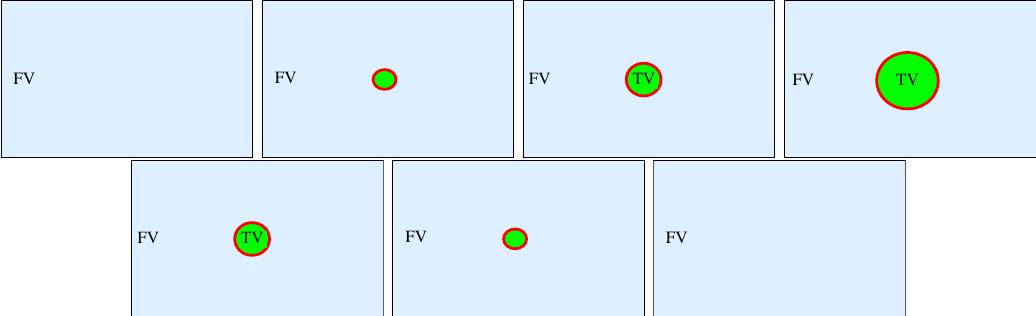
\includegraphics[scale=0.4]{FIGURAS/nucleacion_burbujas}
	\caption{Proceso de nucleación de una burbuja de falso vacío \cite{Masoumi:2015psa}.}
	\label{fig:nucleacionburbujas}
\end{figure}
Analicemos cualitativamente el comportamiento del bounce. Inicialmente, el campo se encuentra en el falso vacío a lo largo de todo el espacio.
%, tal como se indica en la primera condición de frontera \eqref{eq:cond_frontera_qft1}. 
En un cierto instante de tiempo euclideano y en una cierta región del espacio, el campo decae al verdadero vacío mientras que lejos de este, permanece inafectado. Es decir, aparece una burbuja de verdadero vacío 
%tal como se puede ver en la figura , %insertar figura
que empieza a crecer hasta alcanzar su tamaño máximo en $\tau = 0$, a partir del cual se encoge hasta desaparecer, regresando finalmente a la configuración inicial. Todo este proceso se ilustra en la figura \eqref{fig:nucleacionburbujas}
%Este proceso 
y es análogo al proceso de nucleación de burbujas de vapor en la Mecánica Estadística \cite{coleman1977fate}, razón por la cual al bounce también se le denomina burbuja. 

Como es de esperarse, la ecuación de movimiento \eqref{eq:eom_phi} cuenta con una solución trivial que, de acuerdo con la condición de frontera en \eqref{eq:cond_frontera_qft1}, está dada por
\begin{equation} \label{eq:phi_trivial}
	\phi_{\text{FV}}\qty(\tau, \vb{x}) = \phi_+.
\end{equation}
%Tal como se expuso en el párrafo anterior, las soluciones no triviales 

Las ecuación de movimiento \eqref{eq:eom_phi}, las condiciones de frontera \eqref{eq:cond_frontera_qft1} y \eqref{eq:cond_frontera_qft3} y la interpretación del bounce como una burbuja de verdadero vacío, sugieren asumir que este último cuenta con una simetría $O\qty(4)$, es decir, es invariante ante rotaciones del espaciotiempo euclideano o esféricamente simétrico \cite{weinberg2012classical}. Para una gran cantidad de potenciales, esto siempre es posible 
%encontrar un bounce de esta forma 
\cite{coleman1978action}. 

Introduzcamos la distancia euclideana
\begin{equation}
	\rho^2 \equiv \tau^2 + \vb{x}^2
\end{equation}
de tal manera que, de acuerdo con lo establecido anteriormente,  $\phi = \phi\qty(\rho)$. 
%mientras que \eqref{eq:cond_frontera_qft2},
%\begin{equation}
%\eval{\pdv{\phi\qty(\rho)}{\tau}}_{\tau = 0} = 0.
%\end{equation}
%Como $\rho = \rho(\vb{x}, \tau)$, tenemos que
%\begin{equation}
%\pdv{\phi\qty(\rho)}{\tau} = \dv{\phi}{\rho}\pdv{\rho}{\tau}.
%\end{equation}
%
%\begin{align}
%	2\rho \pdv{\rho}{\tau} &= 2\tau \\
%	\pdv{\rho}{\tau} &= \frac{\tau}{\rho}
%\end{align}
%\begin{equation}
%\eval{\dv{\phi\qty(\rho)}{\tau}}_{\rho = 0} = 0
%\end{equation}
%\begin{equation}
%\eval{\dv{\phi}{\rho}}_{\rho = 0} = 0
%\end{equation}
Resulta conveniente renombrar $\tau = x_4$ de tal manera que 
\begin{equation} \label{eq:rho_xi}
	\rho^2 = \sum_{i = 1}^{4} x_i^2.
\end{equation}
%donde $\vb{x} = \qty(x, y, z) = \qty(x_1, x_2, x_3)$. 
De acuerdo con esta notación, la ecuación de movimiento \eqref{eq:eom_phi} está dada por
\begin{equation} \label{eq:eom_xi}
\sum_{i = 1}^{4} \pdv[2]{\phi\qty(\rho)}{x_i} = U'\qty(\phi).
\end{equation}
Escrita de esa manera obtendremos 
%fácilmente la ecuación de movimiento para 
la correspondiente a $\phi\qty(\rho)$. 
%nos facilitará el cambio de variable. 
Haciendo uso de la regla de la cadena, 
\begin{equation} \label{eq:dv_phi_rho}
	\pdv{\phi\qty(\rho)}{x_i} = \dv{\phi}{\rho}\pdv{\rho}{x_i}.
%	&= \frac{x_i}{\rho}\dv{\phi}{\rho}.
\end{equation}
Derivando \eqref{eq:rho_xi} respecto a $x_i$,
\begin{align}
2\rho \pdv{\rho}{x_i} &= 2x_i \\ \label{eq:dv_rho_xi}
\pdv{\rho}{x_i} &= \frac{x_i}{\rho}
\end{align}
y reemplazando esta última
%\eqref{eq:dv_rho_xi} 
en \eqref{eq:dv_phi_rho}, 
\begin{equation} \label{eq:dv_phi_rho2}
\pdv{\phi\qty(\rho)}{x_i} = \frac{x_i}{\rho}\dv{\phi}{\rho}.
\end{equation}
Derivando la ecuación anterior
%\eqref{eq:dv_phi_rho2} 
respecto a $x_i$ y usando nuevamente \eqref{eq:dv_rho_xi},
\begin{align}
	\pdv[2]{\phi\qty(\rho)}{x_i} &= \frac{x_i}{\rho}\dv[2]{\phi}{\rho}\pdv{\rho}{x_i} + \qty(\frac{1}{\rho} - \frac{x_i}{\rho^2}\pdv{\rho}{x_i})\dv{\phi}{\rho} \\
	&= \frac{x_i^2}{\rho^2}\dv[2]{\phi}{\rho} + \frac{1}{\rho}\qty(1 - \frac{x_i^2}{\rho^2})\dv{\phi}{\rho}. 
\end{align}
Por último, sumamos las derivadas,
\begin{align}
\sum_{i = 1}^{4} \pdv[2]{\phi\qty(\rho)}{x_i} &=  \frac{\sum_{i = 1}^{4} x_i^2}{\rho^2}\dv[2]{\phi}{\rho} + \frac{1}{\rho}\qty(4 - \frac{\sum_{i = 1}^{4} x_i^2}{\rho^2})\dv{\phi}{\rho}, 
\end{align}
y simplificamos haciendo uso de \eqref{eq:rho_xi} para obtener finalmente la ecuación de movimiento 
%en términos de $\phi\qty(\rho)$
\begin{equation} \label{eq:eom_rho}
	\dv[2]{\phi}{\rho} + \frac{3}{\rho}\dv{\phi}{\rho} = U'\qty(\phi).
\end{equation}

Las condiciones de frontera \eqref{eq:cond_frontera_qft1} y \eqref{eq:cond_frontera_qft3} se reducen a 
\begin{equation} \label{eq:cond_frontera_rho1}
\lim_{\rho \rightarrow \pm\infty} \phi\qty(\rho) = \phi_+.
\end{equation}
Con la finalidad de evitar que las soluciones cuenten con una singularidad en el origen, requerimos que \cite{coleman1977fate}
\begin{equation}
	\eval{\dv{\phi}{\rho}}_0 = 0.
\end{equation}

La ecuación de movimiento \eqref{eq:eom_rho} puede ser interpretada como la ecuación de movimiento de una partícula 

%analisis clasico de la eom
%argumento overshoot-undershoot de la existencia de la solucion

\subsection{Aproximación de la pared delgada}

El campo dentro de la burbuja, en realidad corresponde al punto de retorno y no al verdadero vacío \cite{lee2005fate}. 

\section{Cálculo de la tasa de decaimiento del falso vacío por unidad de volumen}

Habiendo obtenido las configuraciones clásicas relevantes en el decaimiento del falso vacío, procedemos al cálculo de la tasa de decaimiento del falso vacío por unidad de volumen $\Gamma/V$. Siguiendo el formalismo de Coleman y Callan, partimos de la amplitud de transición 
\begin{equation}
I = \bra{\phi_f}e^{-HT/\hbar}\ket{\phi_i} = \int \mathcal{D}\phi \, e^{-S_E\qty[\phi\qty(\vb{x},\tau)]/\hbar}.
\end{equation}
De acuerdo con la condición de frontera \eqref{eq:cond_frontera_qft1}, $\phi_i = \phi_f = \phi_+$.

Las burbujas de falso vacío pueden aparecer en cualquier región del espacio, es decir, son invariantes ante translaciones espaciales \cite{coleman1977fate}. 

Es posible demostrar que el modo negativo es único para todos los casos de interés \cite{coleman1977fate, coleman1988quantum}

\section{El destino del falso vacío}

\subsection{Implicaciones cosmológicas}

\subsection{Aplicaciones}
\chapter{Conclusiones}

Si bien hemos podido calcular la tasa de decaimiento $\Gamma$ para el decaimiento del falso vacío, quedan varias preguntas conceptuales que no podrán ser abordadas en este trabajo de investigación y que tampoco se discuten a profundidad en la literatura consultada. Por ejemplo, la hermiticidad 

Por último, pero no por eso menos importante, el presente trabajo de investigación representa una pequeña contribución a la literatura en español sobre el decaimiento del falso vacío y espero puede ser utilizada como referencia en investigaciones futuras. 

\printbibliography
\addcontentsline{toc}{chapter}{Bibliografía}

\end{document}